\documentclass{article}
\usepackage{graphicx}
\usepackage{amsmath}
\usepackage[parfill]{parskip}
\usepackage{hyperref}
\graphicspath{ {./figures/} }

\title{COMP.SEC.220 Security Protocol\footnote{github --- \url{https://github.com/ancuongnguyen07/SecurityProtocol}}}
\author{Cuong Nguyen --- LAB 4}
\date{22/09/2022}

\begin{document}
    
\maketitle

\section*{Exercise 1}

\subsection*{Task 1}
%
\begin{itemize}
    \item Alice sends Bob \(A = g^{a} \mod p: 4 = 7^{6} \mod 11\)
    \item Bobs sends Alice \(B = g^{a} \mod p: 8 = 7^{9}  \mod 11\)
    \item Alice computes \(s = B^{a} \mod p: 3 = 8^{6} \mod 11\)
    \item Bobs computes \(s = A^{b} \mod p: 3 = 4^{9} \mod 11\)
    \item Now Bobs and Alice share the final key \(s = 3\)
\end{itemize}

\subsection*{Task 2 + 3}
%
Because g = 5 is the primitive root of p = 47, we can solve \(Y = g^{b}
\mod p\ or\ 3 = 5^{b} \mod 47\) in 46 trials. Running a simple for-loop,
I found that the value of \emph{b} is 20. So the shared key is:
\begin{align*}
    s &= X^{b} \mod p \\
    2 &= 38^{20} \mod 47
\end{align*}
After running the Caesar decryption script with shift key 2, I obtained:
\begin{center}
    \textbf{YOU HAVE REACHED A NEW LEVEL --- ADMIN}
\end{center}

\section*{Exercise 2}
%


\section*{Exercise 3}
%
\begin{figure}
    \centering
    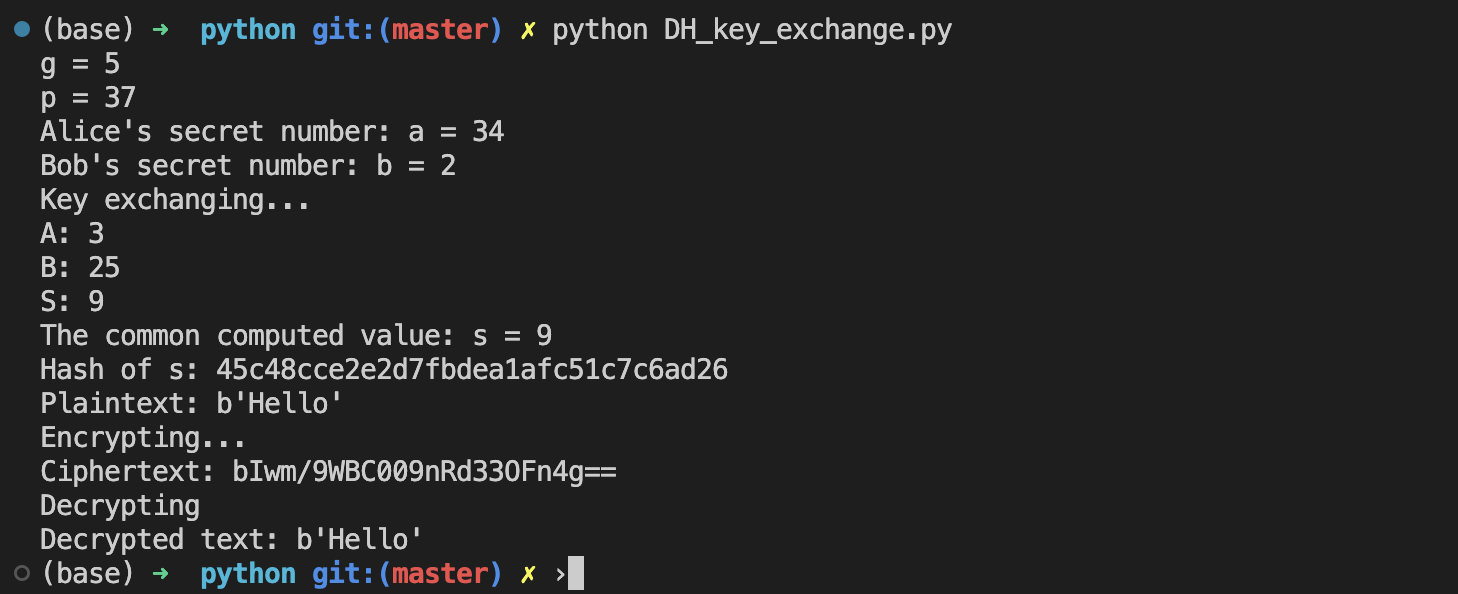
\includegraphics[width=\textwidth, height=\textheight, keepaspectratio]{DH_implementation.png}
    \caption{DH-implementation Python program}
\end{figure}

\textbf{The security of a D-H key exchange protocol is based on?}\\
It's based on the choice of \emph{g} and \emph{p}.

\textbf{The D-H key exchange protocol is vulnerable to?}\\
It is vulnerable to a man-inthe-middle-attack as it doesn't provide
any authentication of the communicating parties.

\textbf{What is the condition for selecting a good value of o in a D-H key exchange protocol?}\\
The order of \emph{p} should have a large prime factor. It is sometimes
calculated as \(p = 2q + 1\), since the order of \emph{p} is then only dvisible
by 2 and \emph{q}.

\end{document}